\documentclass[border=1pt]{standalone}
\usepackage[dvipsnames]{xcolor}
\usepackage{tikz}                       % Graphen und kommutative Diagramme
\usetikzlibrary{patterns}               % Um schraffierte Formen in der tikzpicture-Umgebung zu zeichnen.


\begin{document}
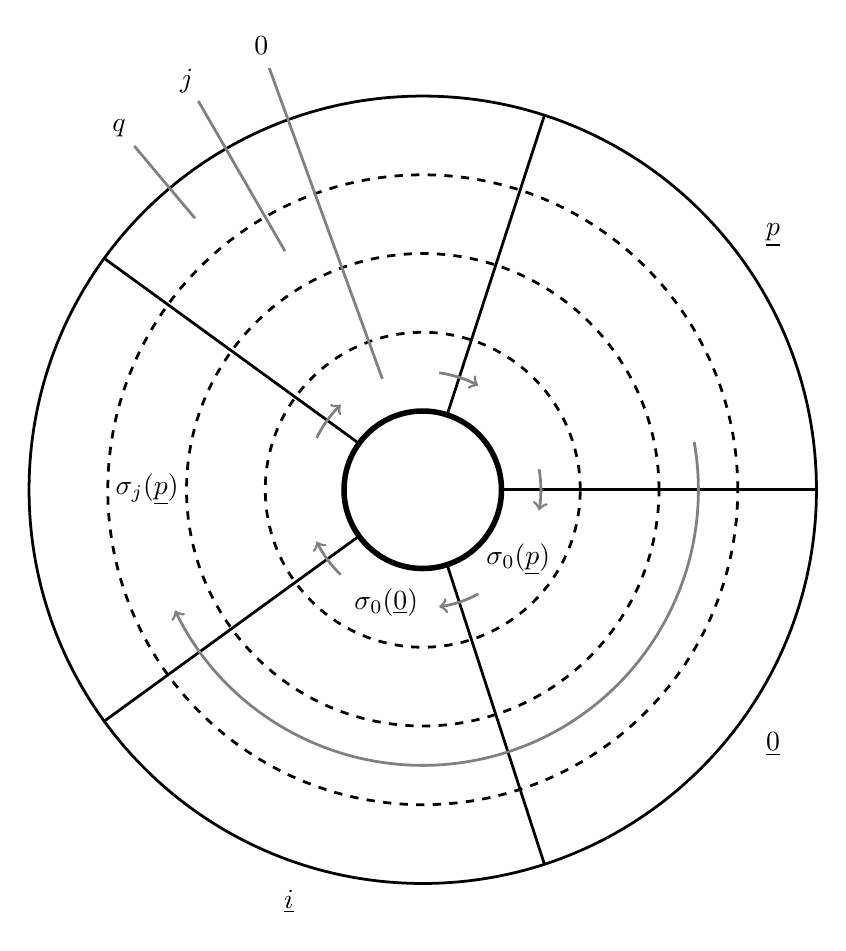
\begin{tikzpicture}[line width=1pt]

\newcommand{\ul}{\underline}

% draw inner and outer circles
\draw[color=black, line width=2pt] (0, 0) circle (1);
\draw[color=black] (0, 0) circle (5);

% draw dashed circles
\foreach \i in {2,...,4}
{
    \draw[color=black, dashed] (0, 0) circle (\i);
}

% draw radial segment
\foreach \i in {0,...,4}
{
		\draw (\i * 72 : 1) -- (\i * 72 : 5);
}

%draw nodes
\draw node at (110 : 6) {$0$};
\draw[color=black!50] (110 : 5.7) -- (110 : 1.5);
\draw node at (120 : 6) {$j$};
\draw[color=black!50] (120 : 5.7) -- (120 : 3.5);
\draw node at (130 : 6) {$q$};
\draw[color=black!50] (130 : 5.7) -- (130 : 4.5);

\draw node at (72 * 4 + 36 : 5.5) {$\ul 0$};
\draw node at (72 * 3 + 36 : 5.5) {$\ul i$};
\draw node at (36 : 5.5) {$\ul p$};

% draw sigma_0
\foreach \i in {0,...,4}
{
    \draw[<-, color=black!50] (72 * \i - 10 : 1.5) arc[radius = 1.5, start angle = 72 * \i - 10, delta angle = 20];
}
\draw node at (72 * 4 + 36 : 1.5) {$\sigma_0(\ul p)$};
\draw node at (72 * 3 + 36 : 1.5) {$\sigma_0(\ul 0)$};

% draw sigma_i

\draw node at (2 * 72 + 36 : 3.5) {$\sigma_j(\ul p)$};

\draw[->, color=black!50] (10 : 3.5) arc[radius = 3.5, start angle = 10, delta angle = - 2*72 - 20];

\end{tikzpicture}
\end{document}